\section{ACTION Token}

\subsection{Overview}

The main reason to acquire ACTION is to participate in the creation, gaming, or governance aspects, not for speculative profit.

\subsubsection{Purpose and Utility}
The ACTION Token represents \textbf{ownership} and \textbf{governance} within the Action Substrate. Core uses include:

\begin{itemize}
\item Paying for hyperobject creation, publishing, and registry
\item Facilitating transactions within the marketplace
\item Staking may be used for network security and participation in governance but does not provide financial returns\footnote{The staking mechanism is designed purely for network security and governance participation, not as an investment vehicle. Staked tokens are locked for governance voting power and network validation, but do not generate yield or financial returns, distinguishing ACTION from traditional yield-bearing tokens.}
\item Participating in governance to shape protocol updates and treasury allocations
\item Fostering community expansion and incentivizing activity on Action
\item Extensible utility. As game assets evolve, and the number of people using onchain game assets expands, and ACTION may be utilized in new ways by the community.
\end{itemize}

\subsubsection{Unique Value Proposition}
\begin{itemize}
\item Directly tied to the growth of sovereign worlds and games on the Action substrate
\item Incorporates treasury mechanisms to fund environmental and social initiatives
\item The Action substrate, leveraging AO's network, may further incentivize security and sovereignty by tying hyperobjects to validated node operation
\end{itemize}

\subsubsection{Implementation}
\begin{itemize}
\item Built and spawned on the audited AO token blueprint
\item Disowned by the deployer at launch
\item ACTION governance will transition over time through an autonomous governance framework, reducing reliance on any single entity
\end{itemize}

\subsection{Distribution and Allocation}

\textbf{Fixed Supply:} 10,000,000,000 ACTION\footnote{The fixed supply of 10 billion tokens was carefully chosen to balance sufficient granularity for microtransactions with the need to maintain scarcity. This number allows for broad distribution across the ecosystem while ensuring each token retains meaningful utility for governance and platform interactions.}

\vspace{0.5em}

\noindent The majority of ACTION tokens (75\%) will be allocated to the communities using Action, and the Broadside and Basejump communities that inspired its creation. Contributors and team receive allocations for contributing work to the ecosystem, not as passive investments expecting a return.


\begin{figure}
\centering
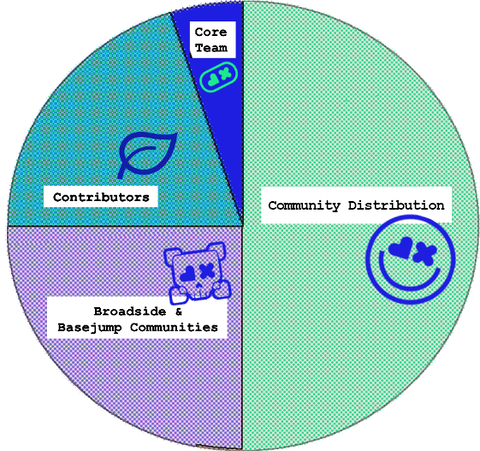
\includegraphics[width=0.8\columnwidth]{images/image7.png}
\vspace{1em}
\caption{ACTION Token Distribution and Allocation}
\label{fig:token_distribution}
\end{figure}

\begin{table}
  \centering
  \renewcommand{\arraystretch}{1.2}
  \caption{ACTION Token Distribution\protect\footnotemark}
  \begin{tabularx}{\columnwidth}{>{\raggedright\arraybackslash}p{0.7\columnwidth}>{\raggedleft\arraybackslash}p{0.2\columnwidth}}
  \hline
  \textbf{Category} & \multicolumn{1}{>{\raggedleft\arraybackslash}p{0.2\columnwidth}}{\textbf{Allocation}} \\
  \hline
  Community Distribution & 50\% \\
  Basejump \& Broadside Ecosystem & 25\% \\
  Contributor (future team, advisors, and investors) & 20\% \\
  Basejump Team & 5\% \\
  \hline
  \end{tabularx}
\end{table}
\footnotetext{Contributors and Team distributions are subject to one year lock and three year schedule}

\subsubsection{Community Distribution (50\%)}
\begin{itemize}
\item 50\% of ACTION tokens will be made available via the Permaweb Index; a new engine for community-driven distribution on AO designed to foster growth across the Permaweb
\item For more on the PermaWeb Index, visit \url{https://ao.arweave.net/}
\item The primary aim is broad usage and decentralization, \textit{not} raising capital
\end{itemize}

\subsubsection{Action, Basejump and Broadside Ecosystem (25\%)}
\begin{itemize}
\item 20\% of ACTION tokens will be reserved for Basejump users and communities, including the Broadside OG community, and allocated as rewards for playing games built on Action, creating new games and assets using Action, and for helping grow the Action ecosystem
\item 5\% of ACTION tokens will be allocated to Broadside OG holders
\item Broadside OGs will also earn the highest multipliers on rewards within the Basejump ecosystem
\item This allocation of ACTION will distribute directly to Broadside OG Action Figures
\end{itemize}

\subsubsection{Contributors (20\%)}
\begin{itemize}
\item We are setting aside 20\% of ACTION token supply for current and future contributors to the development of the Action ecosystem. This includes strategic partners such as Community Labs, as well as potential future contributors, team members and advisors. \cite{Takahashi2023}
\item Contributor allocations are subject to a one year lock and three year distribution schedule
\end{itemize}

\subsubsection{Basejump Team (5\%)}
\begin{itemize}
\item 5\% of tokens is reserved for the core Basejump team, as well as advisors
\item Team allocations are subject to a one year lock and three year distribution schedule
\end{itemize}




\subsection{Economic Model}

\subsubsection{Supply Dynamics}
Fixed supply; total supply is capped for functional reasons (like ensuring consistency across all participants)

\subsubsection{Protocol Fee Flows}
Marketplace fees, hyperobject publishing/registration, direct sales, and compute/persistence fees

\subsubsection{Feedback Loops}
Staking benefits, and usage-based demand tied to ecosystem growth

\begin{figure}[ht]
  \centering
  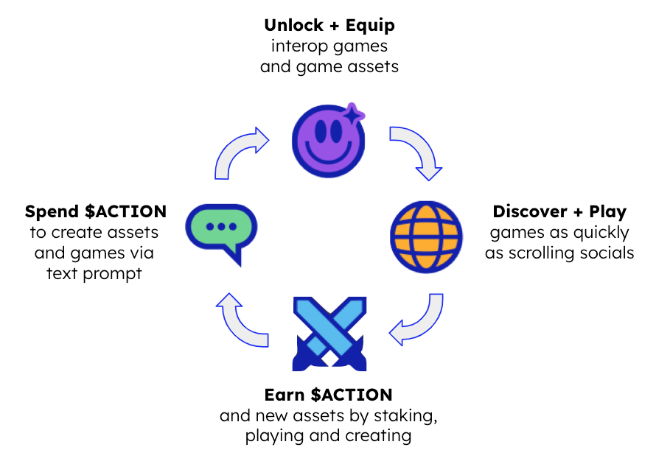
\includegraphics[width=\columnwidth]{images/image8.png}
  \caption{Action is an open-loop system, designed to reward users who play Action-powered games, create games and assets using Action, and help secure the network through staking.}
  \label{fig:economic_model}
\end{figure}
  

\subsection{Implementation}

ACTION's AO process is implemented according to the AO Token Blueprint, with the following standard handlers, as shown in Figure \ref{fig:action_token_interface}.

\begin{figure}[t]
\begin{lstlisting}[basicstyle=\ttfamily\small]
-- Get info about the ACTION token process
Info() -> {
  Name, Ticker, Logo, Denomination
}

-- Get balance of a specific account
Balance(Target?) -> {
  Balance, Ticker, Account, Data
}

-- Get all account balances
Balances() -> {
  Data -- JSON-encoded map
}

-- Emits standard Credit-Notice and Debit-Notice
Transfer(Recipient, Quantity)

-- Not implemented for ACTION
Mint(Quantity: string)

-- Get total supply of the token
Total-Supply() -> {
  Action, Data, Ticker
}

-- Callable only by a holder of ACTION tokens
Burn(Quantity: string)
\end{lstlisting}
\caption{ACTION Token Handler Interfaces (pseudocode): Core methods for querying state and performing transactions in the ACTION token protocol.}
\label{fig:action_token_interface}
\end{figure}
